% A LaTeX template for EXECUTIVE SUMMARY of the MSc Thesis submissions to 
% Politecnico di Milano (PoliMi) - School of Industrial and Information Engineering
%
% S. Bonetti, A. Gruttadauria, G. Mescolini, A. Zingaro
% e-mail: template-tesi-ingind@polimi.it
%
% Last Revision: October 2021
%
% Copyright 2021 Politecnico di Milano, Italy. NC-BY

\documentclass[11pt,a4paper,twocolumn]{article}

%------------------------------------------------------------------------------
%	REQUIRED PACKAGES AND  CONFIGURATIONS
%------------------------------------------------------------------------------
% PACKAGES FOR TITLES
\usepackage{titlesec}
\usepackage{color}

% PACKAGES FOR LANGUAGE AND FONT
\usepackage[utf8]{inputenc}
\usepackage[english]{babel}
\usepackage[T1]{fontenc} % Font encoding

% PACKAGES FOR IMAGES
\usepackage{graphicx}
\usepackage{tikz} % A package for high-quality hand-made figures.
\usetikzlibrary{}
\graphicspath{{./Images/}} % Directory of the images
\usepackage{eso-pic} % For the background picture on the title page
\usepackage{subfig} % Numbered and caption subfigures using \subfloat
\usepackage{caption} % Coloured captions
\usepackage{transparent}

% STANDARD MATH PACKAGES
\usepackage{amsmath}
\usepackage{amsthm}
\usepackage{bm}
\usepackage[overload]{empheq}  % For braced-style systems of equations

% PACKAGES FOR TABLES
\usepackage{tabularx}
\usepackage{longtable} % tables that can span several pages
\usepackage{colortbl}

% PACKAGES FOR ALGORITHMS (PSEUDO-CODE)
\usepackage{algorithm}
\usepackage{algorithmic}

% PACKAGES FOR REFERENCES & BIBLIOGRAPHY
\usepackage[colorlinks=true,linkcolor=black,anchorcolor=black,citecolor=black,filecolor=black,menucolor=black,runcolor=black,urlcolor=black]{hyperref} % Adds clickable links at references
\usepackage{cleveref}
\usepackage[authoryear, square, numbers, sort&compress]{natbib} % Square brackets, citing references with numbers, citations sorted by appearance in the text and compressed
\bibliographystyle{apalike} % You may use a different style adapted to your field

% PACKAGES FOR THE APPENDIX
\usepackage{appendix}

% PACKAGES FOR ITEMIZE & ENUMERATES 
\usepackage{enumitem}

% OTHER PACKAGES
\usepackage{amsthm,thmtools,xcolor} % Coloured "Theorem"
\usepackage{comment} % Comment part of code
\usepackage{fancyhdr} % Fancy headers and footers
\usepackage{lipsum} % Insert dummy text
\usepackage{tcolorbox} % Create coloured boxes (e.g. the one for the key-words)
\usepackage{stfloats} % Correct position of the tables

%-------------------------------------------------------------------------
%	NEW COMMANDS DEFINED
%-------------------------------------------------------------------------
% EXAMPLES OF NEW COMMANDS -> here you see how to define new commands
\newcommand{\bea}{\begin{eqnarray}} % Shortcut for equation arrays
\newcommand{\eea}{\end{eqnarray}}
\newcommand{\e}[1]{\times 10^{#1}}  % Powers of 10 notation
\newcommand{\mathbbm}[1]{\text{\usefont{U}{bbm}{m}{n}#1}} % From mathbbm.sty
\newcommand{\pdev}[2]{\frac{\partial#1}{\partial#2}}
% NB: you can also override some existing commands with the keyword \renewcommand

%----------------------------------------------------------------------------
%	ADD YOUR PACKAGES (be careful of package interaction)
%----------------------------------------------------------------------------
\usepackage{adjustbox}
\usepackage{enumitem}

%----------------------------------------------------------------------------
%	ADD YOUR DEFINITIONS AND COMMANDS (be careful of existing commands)
%----------------------------------------------------------------------------


% Do not change Configuration_files/config.tex file unless you really know what you are doing. 
% This file ends the configuration procedures (e.g. customizing commands, definition of new commands)
% Set the geometric layout of the document
\usepackage{geometry}
\geometry{
  top=3cm,
  left = 2.0cm,
  right = 2.0cm,
  bottom=2cm,
  headheight= 2cm,
  headsep= 0cm,
}
\raggedbottom 

% Create color bluePoli (-> manuale grafica coordinata:  https://www.polimi.it/fileadmin/user_upload/il_Politecnico/grafica-coordinata/2015_05_11_46xy_manuale_grafica_coordinata.pdf)
\definecolor{bluePoli}{cmyk}{0.4,0.1,0,0.4}

% Custom theorem environments
\declaretheoremstyle[
  headfont=\color{bluePoli}\normalfont\bfseries,
  bodyfont=\color{black}\normalfont\itshape,
]{colored}

\captionsetup[figure]{labelfont={color=bluePoli}} % Set colour of the captions
\captionsetup[table]{labelfont={color=bluePoli}} % Set colour of the captions
\captionsetup[algorithm]{labelfont={color=bluePoli}} % Set colour of the captions

\theoremstyle{colored}
\newtheorem{theorem}{Theorem}[section]
\newtheorem{proposition}{Proposition}[section]

% Enhances the features of the standard "table" and "tabular" environments.
\newcommand\T{\rule{0pt}{2.6ex}}
\newcommand\B{\rule[-1.2ex]{0pt}{0pt}}

% Algorithm description
\newcounter{algsubstate}
\renewcommand{\thealgsubstate}{\alph{algsubstate}}
\newenvironment{algsubstates}{
    \setcounter{algsubstate}{0}%
    \renewcommand{\STATE}{%
    \stepcounter{algsubstate}%
    \Statex {\small\thealgsubstate:}\space}
    }{}
    
% Custom theorem environment
\newcolumntype{L}[1]{>{\raggedright\let\newline\\\arraybackslash\hspace{0pt}}m{#1}}
\newcolumntype{C}[1]{>{\centering\let\newline\\\arraybackslash\hspace{0pt}}m{#1}}
\newcolumntype{R}[1]{>{\raggedleft\let\newline\\\arraybackslash\hspace{0pt}}m{#1}}

% Custom itemize environment
\setlist[itemize,1]{label=$\bullet$}
\setlist[itemize,2]{label=$\circ$}
\setlist[itemize,3]{label=$-$}
\setlist{nosep}

% Set separation of columns 
\setlength{\columnsep}{30pt}

% Create command for background pic
\newcommand\BackgroundPic{% Adding background picture
	\put(230,358){
		\parbox[b][\paperheight]{\paperwidth}{%
			\vfill
			\centering
			\transparent{0.4}
			
\includegraphics[width=0.5\paperwidth]{raggiera_polimi.eps}%
			\vfill
}}}

% Set indentation
\setlength\parindent{0pt}

% Custom title commands
\titleformat{\section}
{\color{bluePoli}\normalfont\Large\bfseries}
{\color{bluePoli}\thesection.}{1em}{}
\titlespacing*{\section}
{0pt}{2ex}{1ex}

\titleformat{\subsection}
{\color{bluePoli}\normalfont\large\bfseries}
{\color{bluePoli}\thesubsection.}{1em}{}
\titlespacing*{\subsection}
{0pt}{2ex}{1ex}

% Custom headers and footers
\pagestyle{fancy}
\fancyhf{}
      
\fancyfoot{}
\fancyfoot[C]{\thepage} % page
\renewcommand{\headrulewidth}{0mm} % headrule width
\renewcommand{\footrulewidth}{0mm} % footrule width

\makeatletter
\patchcmd{\headrule}{\hrule}{\color{black}\hrule}{}{} % headrule
\patchcmd{\footrule}{\hrule}{\color{black}\hrule}{}{} % footrule
\makeatother

% -> Create the header
\chead[C]{
\centering
\begin{tcolorbox}[arc=0pt, boxrule=0pt, colback=bluePoli!60, width=\textwidth, colupper=white]
    \textbf{Executive summary} \hfill \textbf{\author}  
\end{tcolorbox}
}

% Insert here the info that will be displayed into your Title page 
% -> title of your work
\renewcommand{\title}{Three-dimensional bin packing with vertical support}
% -> author name and surname
\renewcommand{\author}{Jacopo Libè}
% -> MSc course
\newcommand{\course}{Computer Science and Engineering - Ingegneria Informatica}
% -> advisor name and surname
\newcommand{\advisor}{Prof. Ola Jabali}
% IF AND ONLY IF you need to modify the co-supervisors you also have to modify the file Configuration_files/title_page.tex (ONLY where it is marked)
\newcommand{\firstcoadvisor}{Davide Croci} % insert if any otherwise comment
%\newcommand{\secondcoadvisor}{Name Surname} % insert if any otherwise comment
% -> academic year
\newcommand{\YEAR}{2021-2022}

%-------------------------------------------------------------------------
%	BEGIN OF YOUR DOCUMENT
%-------------------------------------------------------------------------
\begin{document}

%-----------------------------------------------------------------------------
% TITLE PAGE
%-----------------------------------------------------------------------------
% Do not change Configuration_files/TitlePage.tex (Modify it IF AND ONLY IF you need to add or delete the Co-advisors)
% This file creates the Title Page of the document
% DO NOT REMOVE SPACES BETWEEN LINES!

\twocolumn[{\begin{@twocolumnfalse}

    \AddToShipoutPicture*{\BackgroundPic}
    
    \hspace{-0.6cm}
\includegraphics[width=0.6\textwidth]{logo_polimi_ing_indinf.eps}
    
    \vspace{-1mm}
    \fontsize{0.3cm}{0.5cm}\selectfont \bfseries \textsc{\color{bluePoli} Executive Summary of the Thesis}\\
    
    \vspace{-0.2cm}
    \Large{\textbf{\color{bluePoli}{\title}}}\\
    
    \vspace{-0.2cm}
    \fontsize{0.3cm}{0.5cm}\selectfont \bfseries \textsc{\color{bluePoli} Laurea Magistrale in \course}\\
    
    \vspace{-0.2cm}
    \fontsize{0.3cm}{0.5cm} \selectfont \bfseries Author: \textsc{\textbf{\author}}\\
    
    \vspace{-0.4cm}
    \fontsize{0.3cm}{0.5cm}\selectfont \bfseries Advisor: \textsc{\textbf{\advisor}}\\
    
    % if only ONE co-advisor is present:
    \vspace{-0.4cm}
    \fontsize{0.3cm}{0.5cm}\selectfont \bfseries Co-advisor: \textsc{\textbf{\firstcoadvisor}}\\
    % if more than one co-advisors are present:
    %\vspace{-0.4cm}
    %\fontsize{0.3cm}{0.5cm}\selectfont \bfseries Co-advisors: \textsc{\textbf{\firstcoadvisor}}\textsc{\textbf{\secondcoadvisor}}\\
    
    \vspace{-0.4cm}
    \fontsize{0.3cm}{0.5cm}\selectfont \bfseries Academic year: \textsc{\textbf{\YEAR}}
    
    \small \normalfont
    
    \vspace{11pt}
    
    \centerline{\rule{1.0\textwidth}{0.4pt}}
    
    \vspace{15pt}
    \end{@twocolumnfalse}}]
    
    \thispagestyle{plain} % In order to not show the header in the first page

%%%%%%%%%%%%%%%%%%%%%%%%%%%%%%
%%     THESIS MAIN TEXT     %%
%%%%%%%%%%%%%%%%%%%%%%%%%%%%%%



%% \section{Guidelines}
%% \label{sec:guidelines}
%% 
%% The Executive Summary is a critical overview of your thesis
%% with a focus on the main achievements that have emerged from your research.
%% 
%% The Executive Summary should be organized in sections/paragraphs
%% in order to better highlight the major points of your work.
%% The length should range from four to six pages depending on the length of the thesis manuscript.
%% Keep the Executive Summary concise enough to be effective but long enough to allow it to be complete.
%% It should be written after completing the thesis manuscript as a stand-alone independent document
%% of sufficient clarity and detail to ensure that the reader can figure out the overall objectives,
%% the methodology employed and the results/impact of your research.
%% 
%% In writing the Executive Summary, keep in mind that it is not an abstract, it is not a preface,
%% and it is not a random collection of highlights.
%% With a few exceptions, do not simply cut and paste whole sections or paragraphs of the thesis manuscript
%% into a disorganized and cluttered Executive Summary.
%% You should reorganize information to be informative as well as concise.
%% 
%% The Executive Summary could contain a few important equations related to your work.
%% It could also include the most relevant figures and tables taken or elaborated from the thesis manuscript.
%% 
%% You should also include in the Executive Summary the very essential bibliography of your study.
%% The number of selected references should range from three to five depending on the type of work.
%% 
%% The Executive Summary should contain a final section reporting the main conclusions drawn from your research.

%-----------------------------------------------------------------------------
% INTRODUCTION
%-----------------------------------------------------------------------------
\section{Introduction}
\label{sec:introduction}

Recent progress in the digitalization of industrial processes led to a rise in studies on the Three-Dimensional Bin Packing Problem (3D-BPP).
The problem consists in packing a set of three-dimensional items in the minimum number of bins without any overlap.
The 3D-BPP finds many applications in real-world industrial settings, such as loading boxes onto pallets (Pallet Loading Problem) or in containers (Container Loading Problem). 
Studies in the application areas mentioned above have shown that 3D-BPP can be successfully applied to industrial problems as long as it is extended with new practical constraints. 
Many works in the literature state that one of the most important practical constraints is vertical support (\cite{BORTFELDT20131}), i.e., the fact that each item has sufficient support to keep it from falling.
In this thesis, we develop a new extension of the 3D-BPP that ensures vertical support for each item: the Three-Dimensional Bin Packing Problem with Vertical Support (3D-BPPVS).
Similarly to other works in the literature (\cite{GZARA20201062,paquay2016mixed}), we model this property as a constraint on the minimum amount of area or vertices that rest on other items.

Our research stems from the case study of a logistics company in northern Italy.
The company manages large warehouses where automated lines bring boxes to different packing stations, and then they are loaded onto pallets of standard size.
Since the company deals directly with customers' orders, boxes have very different sizes and are usually packed in smaller quantities.
Moreover, the assortment of items to pack is strongly heterogeneous. Therefore, using standard approaches based on layers of homogeneous boxes is impractical.
During the palletization, levels of already packed items are wrapped to ensure the better overall stability of the pallet.
This wrapping procedure requires minimal unused space between items, a property that is measured with a metric called cage ratio.
The cage ratio is the ratio between the volume of the packed items inside a bin and the volume of the cuboid which surrounds them, the cage.
The cage has the same base as the bin and height equal to the highest packed item inside the bin.
The company's current commercial solutions pack items with an average cage ratio of $60\%$, and a target of $70\%$ was set as a baseline for our work.
A visual representation of the cage ratio is shown in \cref{fig:cage_ratio}.

\begin{figure}[h]
    \resizebox{\columnwidth}{!}{%
    

\tikzset{every picture/.style={line width=0.75pt}} %set default line width to 0.75pt        

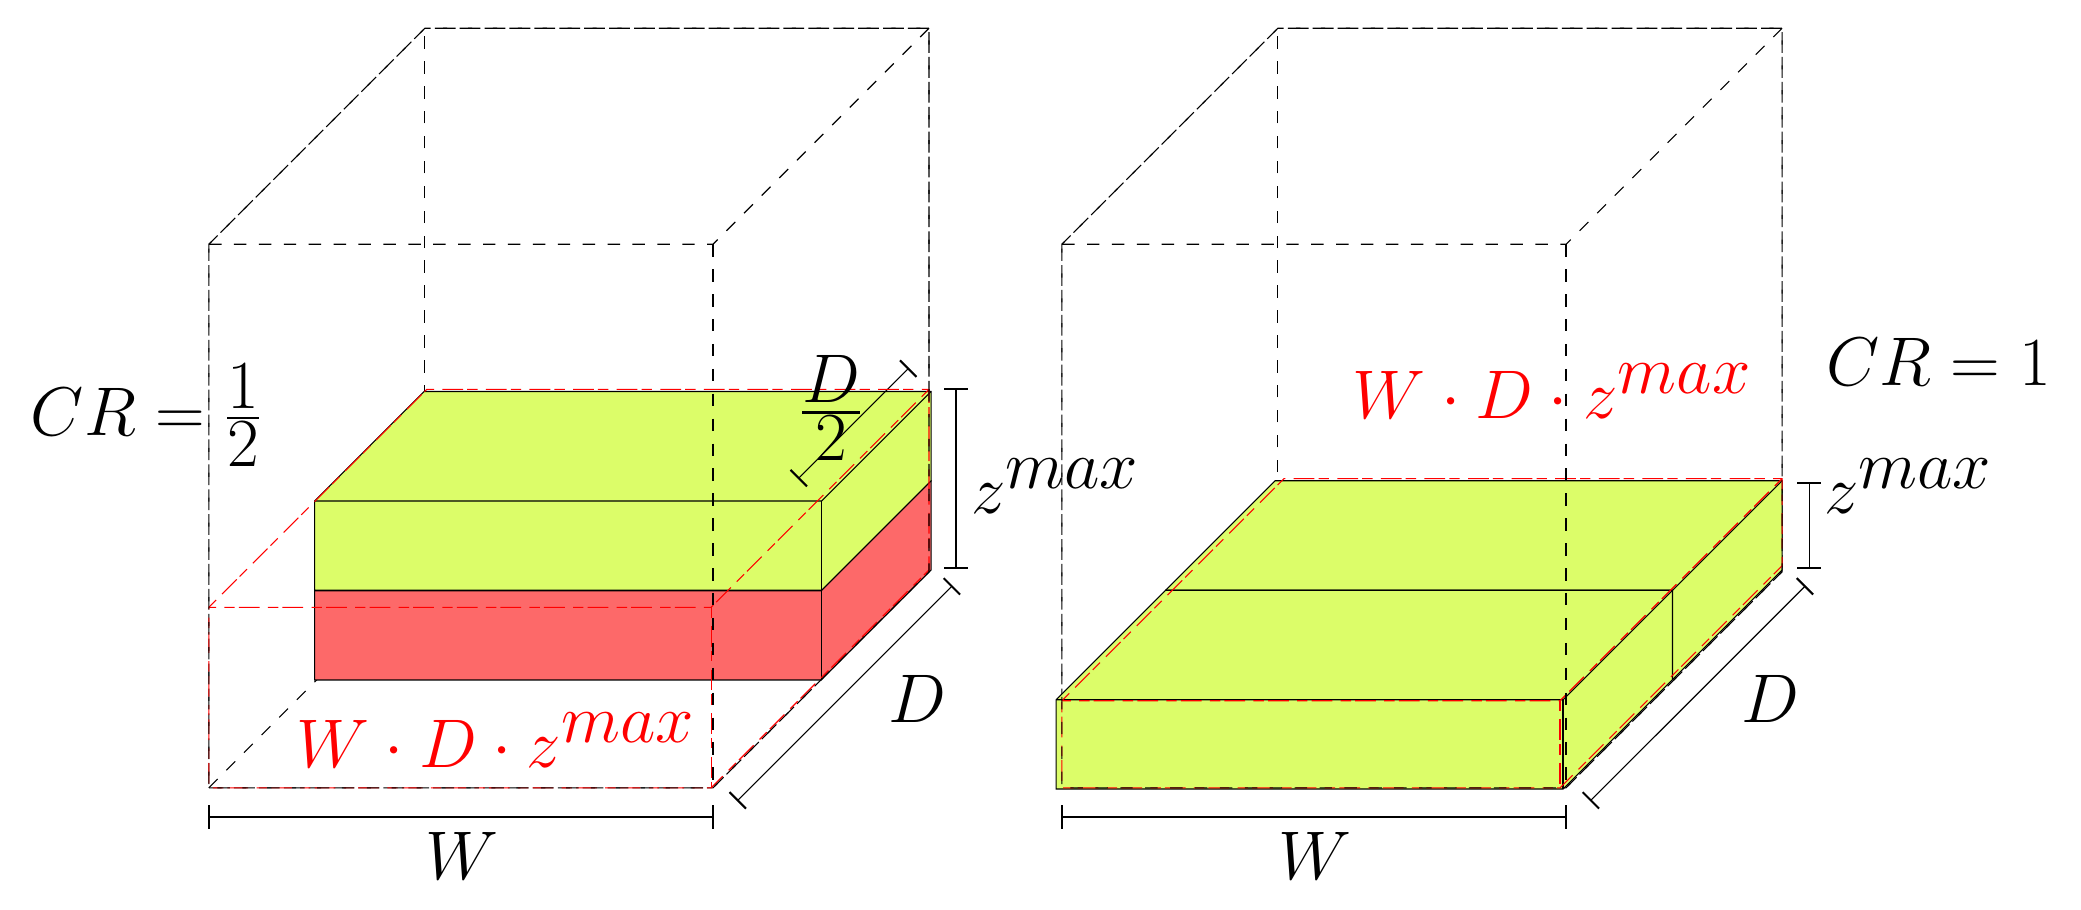
\begin{tikzpicture}[x=0.75pt,y=0.75pt,yscale=-1,xscale=1,font={\fontsize{50pt}{12}\selectfont}]
%uncomment if require: \path (0,479); %set diagram left start at 0, and has height of 479

%Shape: Cube [id:dp9446615397697055] 
\draw  [dash pattern={on 4.5pt off 4.5pt}] (917,301.9) -- (812.9,406) -- (570,406) -- (570,144.1) -- (674.1,40) -- (917,40) -- cycle ; \draw  [dash pattern={on 4.5pt off 4.5pt}] (570,406) -- (674.1,301.9) -- (917,301.9) ; \draw  [dash pattern={on 4.5pt off 4.5pt}] (674.1,301.9) -- (674.1,40) ;
%Shape: Cube [id:dp9924623151681093] 
\draw  [fill={rgb, 255:red, 220; green, 253; blue, 105 }  ,fill opacity=1 ] (620,310.78) -- (672.78,258) -- (917,258) -- (917,301) -- (864.22,353.78) -- (620,353.78) -- cycle ; \draw   (917,258) -- (864.22,310.78) -- (620,310.78) ; \draw   (864.22,310.78) -- (864.22,353.78) ;
%Shape: Cube [id:dp4356357707795666] 
\draw  [fill={rgb, 255:red, 220; green, 253; blue, 105 }  ,fill opacity=1 ] (567.22,363.56) -- (620,310.78) -- (864.22,310.78) -- (864.22,353.78) -- (811.44,406.56) -- (567.22,406.56) -- cycle ; \draw   (864.22,310.78) -- (811.44,363.56) -- (567.22,363.56) ; \draw   (811.44,363.56) -- (811.44,406.56) ;
%Shape: Cube [id:dp900981008021689] 
\draw  [dash pattern={on 4.5pt off 4.5pt}] (506,301.9) -- (401.9,406) -- (159,406) -- (159,144.1) -- (263.1,40) -- (506,40) -- cycle ; \draw  [dash pattern={on 4.5pt off 4.5pt}] (159,406) -- (263.1,301.9) -- (506,301.9) ; \draw  [dash pattern={on 4.5pt off 4.5pt}] (263.1,301.9) -- (263.1,40) ;
%Shape: Cube [id:dp9462720863667783] 
\draw  [fill={rgb, 255:red, 253; green, 105; blue, 105 }  ,fill opacity=1 ] (210,311) -- (263,258) -- (507,258) -- (507,301) -- (454,354) -- (210,354) -- cycle ; \draw   (507,258) -- (454,311) -- (210,311) ; \draw   (454,311) -- (454,354) ;
%Shape: Cube [id:dp20686523528460465] 
\draw  [fill={rgb, 255:red, 220; green, 253; blue, 105 }  ,fill opacity=1 ] (210,267.78) -- (262.78,215) -- (507,215) -- (507,258) -- (454.22,310.78) -- (210,310.78) -- cycle ; \draw   (507,215) -- (454.22,267.78) -- (210,267.78) ; \draw   (454.22,267.78) -- (454.22,310.78) ;
%Straight Lines [id:da9583369995131138] 
\draw    (496,204) -- (443.22,256.78) ;
\draw [shift={(443.22,256.78)}, rotate = 315] [color={rgb, 255:red, 0; green, 0; blue, 0 }  ][line width=0.75]    (0,5.59) -- (0,-5.59)   ;
\draw [shift={(496,204)}, rotate = 315] [color={rgb, 255:red, 0; green, 0; blue, 0 }  ][line width=0.75]    (0,5.59) -- (0,-5.59)   ;
%Straight Lines [id:da4480701288134522] 
\draw    (401.9,420) -- (159,420) ;
\draw [shift={(159,420)}, rotate = 360] [color={rgb, 255:red, 0; green, 0; blue, 0 }  ][line width=0.75]    (0,5.59) -- (0,-5.59)   ;
\draw [shift={(401.9,420)}, rotate = 360] [color={rgb, 255:red, 0; green, 0; blue, 0 }  ][line width=0.75]    (0,5.59) -- (0,-5.59)   ;
%Straight Lines [id:da9761873387202039] 
\draw    (517,308.9) -- (413.86,412) ;
\draw [shift={(413.86,412)}, rotate = 315.01] [color={rgb, 255:red, 0; green, 0; blue, 0 }  ][line width=0.75]    (0,5.59) -- (0,-5.59)   ;
\draw [shift={(517,308.9)}, rotate = 315.01] [color={rgb, 255:red, 0; green, 0; blue, 0 }  ][line width=0.75]    (0,5.59) -- (0,-5.59)   ;
%Straight Lines [id:da1211437330301477] 
\draw    (519,214) -- (519,299.86) ;
\draw [shift={(519,299.86)}, rotate = 270] [color={rgb, 255:red, 0; green, 0; blue, 0 }  ][line width=0.75]    (0,5.59) -- (0,-5.59)   ;
\draw [shift={(519,214)}, rotate = 270] [color={rgb, 255:red, 0; green, 0; blue, 0 }  ][line width=0.75]    (0,5.59) -- (0,-5.59)   ;
%Shape: Cube [id:dp6016430781165488] 
\draw  [color={rgb, 255:red, 255; green, 0; blue, 0 }  ,draw opacity=1 ][dash pattern={on 3.75pt off 3pt on 7.5pt off 1.5pt}] (159,319) -- (264,214) -- (506,214) -- (506,301) -- (401,406) -- (159,406) -- cycle ; \draw  [color={rgb, 255:red, 255; green, 0; blue, 0 }  ,draw opacity=1 ][dash pattern={on 3.75pt off 3pt on 7.5pt off 1.5pt}] (506,214) -- (401,319) -- (159,319) ; \draw  [color={rgb, 255:red, 255; green, 0; blue, 0 }  ,draw opacity=1 ][dash pattern={on 3.75pt off 3pt on 7.5pt off 1.5pt}] (401,319) -- (401,406) ;
%Shape: Cube [id:dp9858212525551202] 
\draw  [dash pattern={on 4.5pt off 4.5pt}] (159,144.1) -- (263.1,40) -- (506,40) -- (506,301.9) -- (401.9,406) -- (159,406) -- cycle ; \draw  [dash pattern={on 4.5pt off 4.5pt}] (506,40) -- (401.9,144.1) -- (159,144.1) ; \draw  [dash pattern={on 4.5pt off 4.5pt}] (401.9,144.1) -- (401.9,406) ;
%Straight Lines [id:da4537070040642701] 
\draw    (812.9,420) -- (570,420) ;
\draw [shift={(570,420)}, rotate = 360] [color={rgb, 255:red, 0; green, 0; blue, 0 }  ][line width=0.75]    (0,5.59) -- (0,-5.59)   ;
\draw [shift={(812.9,420)}, rotate = 360] [color={rgb, 255:red, 0; green, 0; blue, 0 }  ][line width=0.75]    (0,5.59) -- (0,-5.59)   ;
%Straight Lines [id:da13051427322471099] 
\draw    (928,308.9) -- (824.86,412) ;
\draw [shift={(824.86,412)}, rotate = 315.01] [color={rgb, 255:red, 0; green, 0; blue, 0 }  ][line width=0.75]    (0,5.59) -- (0,-5.59)   ;
\draw [shift={(928,308.9)}, rotate = 315.01] [color={rgb, 255:red, 0; green, 0; blue, 0 }  ][line width=0.75]    (0,5.59) -- (0,-5.59)   ;
%Straight Lines [id:da38828166025774113] 
\draw    (930,259) -- (930,299.86) ;
\draw [shift={(930,299.86)}, rotate = 270] [color={rgb, 255:red, 0; green, 0; blue, 0 }  ][line width=0.75]    (0,5.59) -- (0,-5.59)   ;
\draw [shift={(930,259)}, rotate = 270] [color={rgb, 255:red, 0; green, 0; blue, 0 }  ][line width=0.75]    (0,5.59) -- (0,-5.59)   ;
%Shape: Cube [id:dp33203292048167843] 
\draw  [color={rgb, 255:red, 255; green, 0; blue, 0 }  ,draw opacity=1 ][dash pattern={on 3.75pt off 3pt on 7.5pt off 1.5pt}] (570,364) -- (677,257) -- (917,257) -- (917,299) -- (810,406) -- (570,406) -- cycle ; \draw  [color={rgb, 255:red, 255; green, 0; blue, 0 }  ,draw opacity=1 ][dash pattern={on 3.75pt off 3pt on 7.5pt off 1.5pt}] (917,257) -- (810,364) -- (570,364) ; \draw  [color={rgb, 255:red, 255; green, 0; blue, 0 }  ,draw opacity=1 ][dash pattern={on 3.75pt off 3pt on 7.5pt off 1.5pt}] (810,364) -- (810,406) ;
%Shape: Cube [id:dp6959350788468752] 
\draw  [dash pattern={on 4.5pt off 4.5pt}] (570,144.1) -- (674.1,40) -- (917,40) -- (917,301.9) -- (812.9,406) -- (570,406) -- cycle ; \draw  [dash pattern={on 4.5pt off 4.5pt}] (917,40) -- (812.9,144.1) -- (570,144.1) ; \draw  [dash pattern={on 4.5pt off 4.5pt}] (812.9,144.1) -- (812.9,406) ;

% Text Node
\draw (442,196.4) node [anchor=north west][inner sep=0.75pt]    {$\frac{D}{2}$};
% Text Node
\draw (262,426.4) node [anchor=north west][inner sep=0.75pt]    {$W$};
% Text Node
\draw (485,350.4) node [anchor=north west][inner sep=0.75pt]    {$D$};
% Text Node
\draw (72,200.4) node [anchor=north west][inner sep=0.75pt]    {$CR=\frac{1}{2}$};
% Text Node
\draw (525,246.4) node [anchor=north west][inner sep=0.75pt]    {$z^{max}$};
% Text Node
\draw (200,368.4) node [anchor=north west][inner sep=0.75pt]  [color={rgb, 255:red, 255; green, 0; blue, 0 }  ,opacity=1 ]  {$W\cdot D\cdot z^{max}$};
% Text Node
\draw (673,426.4) node [anchor=north west][inner sep=0.75pt]    {$W$};
% Text Node
\draw (896,350.4) node [anchor=north west][inner sep=0.75pt]    {$D$};
% Text Node
\draw (937,188.4) node [anchor=north west][inner sep=0.75pt]    {$CR=1$};
% Text Node
\draw (936,246.4) node [anchor=north west][inner sep=0.75pt]    {$z^{max}$};
% Text Node
\draw (709,200.4) node [anchor=north west][inner sep=0.75pt]  [color={rgb, 255:red, 255; green, 0; blue, 0 }  ,opacity=1 ]  {$W\cdot D\cdot z^{max}$};


\end{tikzpicture}

    }
    \caption{Cage ratio of two different bin configurations}
    \label{fig:cage_ratio}
\end{figure}

In this thesis we
\begin{itemize}
    \item formulate a mixed-integer linear programming model for the 3D-BPPVS with a discretized version of the support constraint,
    \item develop a constructive heuristic that fills bins while guaranteeing vertical support, without explicitly building layered solutions,
    \item introduce a beam search heuristic that expands the constructive heuristic's solution space by exploring different orders of item palletization,
    \item validate the proposed heuristic against our model and against the most relevant heuristics from the 3D-BPP literature,
    \item generate and share a data set based on real-world instances that we use to benchmark our heuristic.
\end{itemize}

\section{Literature Review}
The 3D-BPP is the generalization of the one-dimensional bin packing problem, which is NP-Hard (\cite{martello2000three}).
Exact methods can only solve small instances of the problem, which means that most solutions proposed in the literature are heuristics.
Heuristics for the 3D-BPP are designed to solve the standard problem and do not consider practical constraints.
\cite{martello2000three} provided a set of benchmark instances for 3D-BPP heuristics and an exact method based on a two-level branch-and-bound algorithm.
Their method used a staircase placement strategy, where a series of corner points were identified as possible placement points to evaluate.
The method was later extended in \cite{crainic2008extreme} to find new placement niches that were previously ignored, introducing the concept of Extreme Points.
\cite{gonccalves2013biased} introduced a biased random-key genetic algorithm (BRKGA) for the 3D-BPP, which is one of the best-performing heuristics on the benchmark instances of \cite{martello2000three}.
Their algorithm was later extended in \cite{zudio2018brkga} by incorporating a variable neighborhood descent procedure, which improved the number of generations needed to find high-quality results.

The concept of vertical support received most of its contribution from the literature on Container Loading Problems (CLP) and Pallet Loading Problems (PLP).
As noted in \cite{BORTFELDT20131}, static stability is usually implicitly enforced as a consequence of load compactness or explicitly guaranteed by using filler material in a post-processing step.
Most heuristics for CLPS and PLPs try to build dense layers composed of similar items that they stack, reducing the problem to a one-dimensional bin packing problem.
Layers are filtered based on the fill rate, and when they are below a certain threshold, they are discarded (e.g., \cite{elhedhli2019three, Alonso2020}).
When no new layer can be built, new bins are opened, simpler placement methods are used to pack the remaining items, or filler material is used to complete the layers.

Our solution to the problem fills the gap in the research by finding solutions to the 3D-BPPVS without explicitly building layers, and without the use of filler material.

\section{Proposed Solution}

Based on other publications from the literature and on our case study partner's insights, we state that an item is vertically supported if one of the following conditions holds.

\begin{enumerate}[label={\textbf{Condition \arabic*}.},ref={\arabic*},leftmargin=*]
    \item the percentage of base area that leans on other items is larger than a predetermined threshold $\alpha_s$. \label{support:area_support}
    \item the number of vertices resting on other items is greater than or equal to 3, and Condition \ref{support:area_support} is met with a smaller threshold $\alpha^\prime_s$. \label{support:vertex_support}
\end{enumerate}
We consider two items to be of equal height if their heights do not differ more than a tolerance threshold $\beta_s$
A visual representation of both support conditions is presented in \cref{fig:support}.

\begin{figure}[h]
    \resizebox{\columnwidth}{!}{%
    

\tikzset{every picture/.style={line width=0.75pt}} %set default line width to 0.75pt        

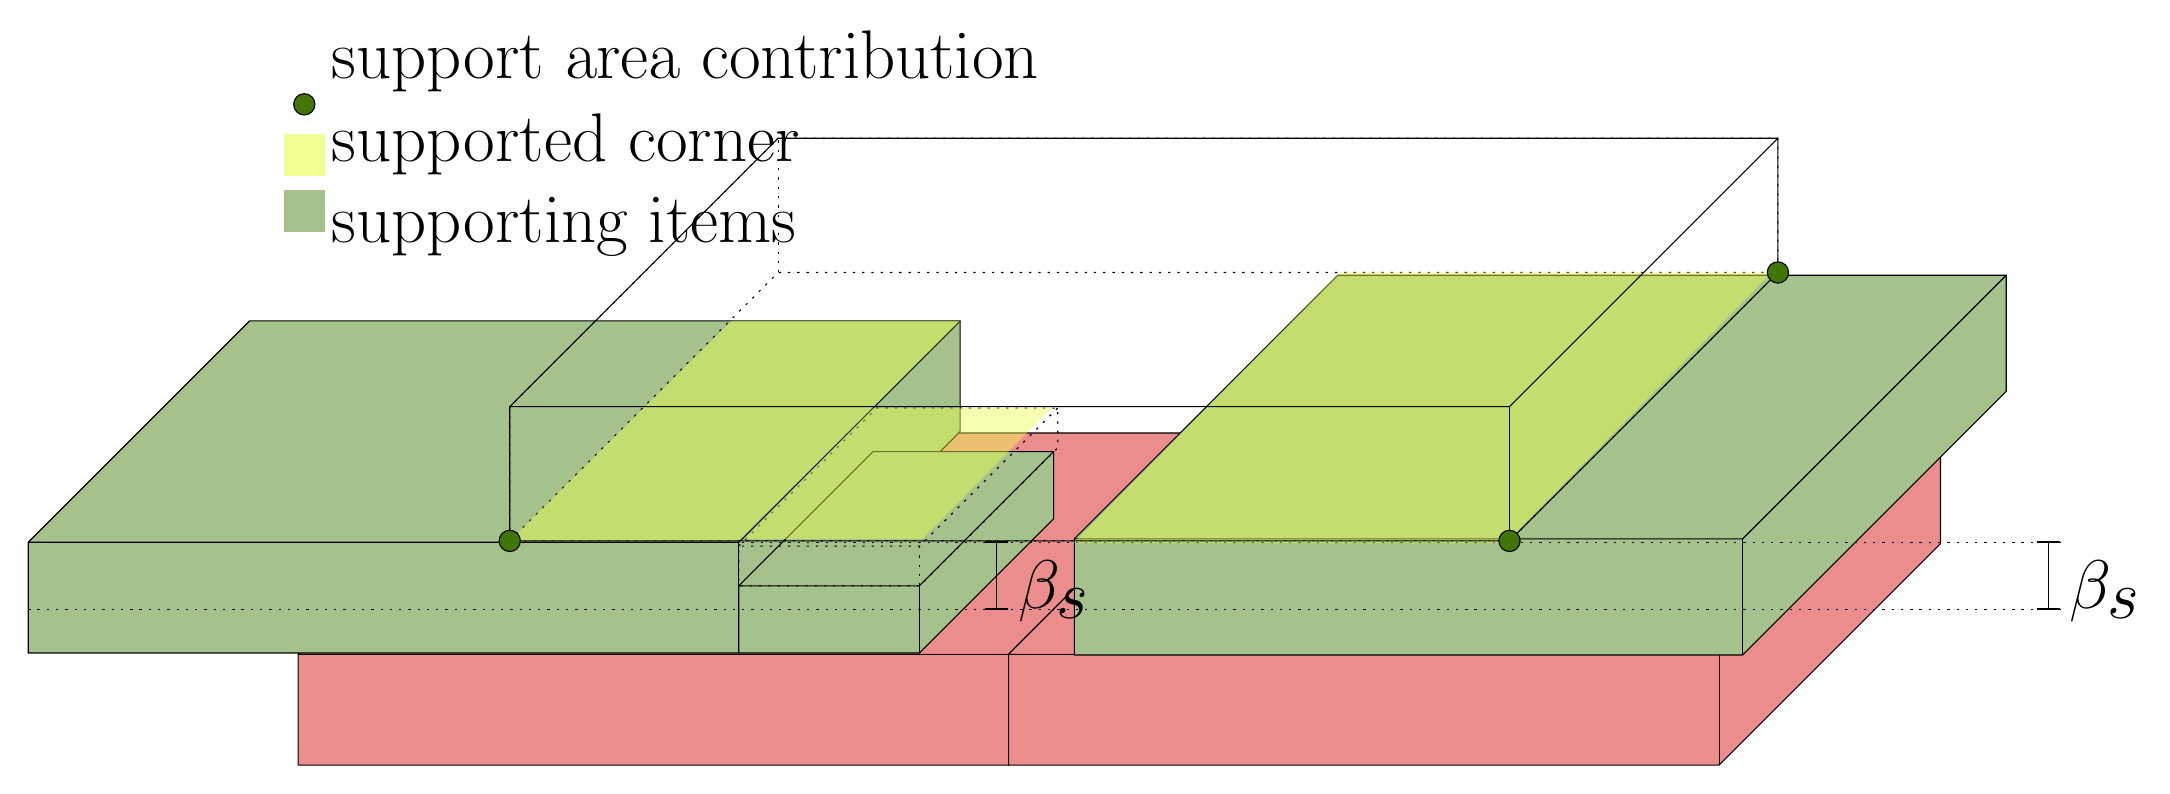
\begin{tikzpicture}[x=0.75pt,y=0.75pt,yscale=-1,xscale=1,font={\fontsize{50pt}{12}\selectfont}]
%uncomment if require: \path (0,479); %set diagram left start at 0, and has height of 479

%Shape: Cube [id:dp9411979483763162] 
\draw  [fill={rgb, 255:red, 236; green, 141; blue, 141 }  ,fill opacity=1 ] (194,306.67) -- (300.67,200) -- (643,200) -- (643,253.33) -- (536.33,360) -- (194,360) -- cycle ; \draw   (643,200) -- (536.33,306.67) -- (194,306.67) ; \draw   (536.33,306.67) -- (536.33,360) ;
%Shape: Cube [id:dp993645103603593] 
\draw  [fill={rgb, 255:red, 236; green, 141; blue, 141 }  ,fill opacity=1 ] (536.33,306.67) -- (643,200) -- (985.33,200) -- (985.33,253.33) -- (878.67,360) -- (536.33,360) -- cycle ; \draw   (985.33,200) -- (878.67,306.67) -- (536.33,306.67) ; \draw   (878.67,306.67) -- (878.67,360) ;
%Shape: Cube [id:dp23986673546182513] 
\draw  [fill={rgb, 255:red, 165; green, 194; blue, 140 }  ,fill opacity=1 ] (64,252.67) -- (170.67,146) -- (513,146) -- (513,199.33) -- (406.33,306) -- (64,306) -- cycle ; \draw   (513,146) -- (406.33,252.67) -- (64,252.67) ; \draw   (406.33,252.67) -- (406.33,306) ;
%Shape: Cube [id:dp5474008601617114] 
\draw  [fill={rgb, 255:red, 165; green, 194; blue, 140 }  ,fill opacity=1 ] (406.33,273.67) -- (471,209) -- (558,209) -- (558,241.33) -- (493.33,306) -- (406.33,306) -- cycle ; \draw   (558,209) -- (493.33,273.67) -- (406.33,273.67) ; \draw   (493.33,273.67) -- (493.33,306) ;
%Shape: Cube [id:dp7313777533771082] 
\draw  [fill={rgb, 255:red, 165; green, 194; blue, 140 }  ,fill opacity=1 ] (568,251) -- (695,124) -- (1017,124) -- (1017,180) -- (890,307) -- (568,307) -- cycle ; \draw   (1017,124) -- (890,251) -- (568,251) ; \draw   (890,251) -- (890,307) ;
%Shape: Cube [id:dp9978562503762016] 
\draw  [dash pattern={on 0.84pt off 2.51pt}] (907,122.67) -- (777.67,252) -- (296,252) -- (296,187.33) -- (425.33,58) -- (907,58) -- cycle ; \draw  [dash pattern={on 0.84pt off 2.51pt}] (296,252) -- (425.33,122.67) -- (907,122.67) ; \draw  [dash pattern={on 0.84pt off 2.51pt}] (425.33,122.67) -- (425.33,58) ;
%Shape: Cube [id:dp48964002783685845] 
\draw  [color={rgb, 255:red, 0; green, 0; blue, 0 }  ,draw opacity=1 ][fill={rgb, 255:red, 255; green, 255; blue, 255 }  ,fill opacity=0 ][dash pattern={on 0.84pt off 2.51pt}] (406.33,254.53) -- (472.86,188) -- (560,188) -- (560,207.14) -- (493.47,273.67) -- (406.33,273.67) -- cycle ; \draw  [color={rgb, 255:red, 0; green, 0; blue, 0 }  ,draw opacity=1 ][dash pattern={on 0.84pt off 2.51pt}] (560,188) -- (493.47,254.53) -- (406.33,254.53) ; \draw  [color={rgb, 255:red, 0; green, 0; blue, 0 }  ,draw opacity=1 ][dash pattern={on 0.84pt off 2.51pt}] (493.47,254.53) -- (493.47,273.67) ;
%Straight Lines [id:da26590658600836115] 
\draw    (1037.33,252.67) -- (1037.33,285) ;
\draw [shift={(1037.33,285)}, rotate = 270] [color={rgb, 255:red, 0; green, 0; blue, 0 }  ][line width=0.75]    (0,5.59) -- (0,-5.59)   ;
\draw [shift={(1037.33,252.67)}, rotate = 270] [color={rgb, 255:red, 0; green, 0; blue, 0 }  ][line width=0.75]    (0,5.59) -- (0,-5.59)   ;
%Straight Lines [id:da26590658600836116] 
\draw    (530.33,252.67) -- (530.33,285) ;
\draw [shift={(530.33,285)}, rotate = 270] [color={rgb, 255:red, 0; green, 0; blue, 0 }  ][line width=0.75]    (0,5.59) -- (0,-5.59)   ;
\draw [shift={(530.33,252.67)}, rotate = 270] [color={rgb, 255:red, 0; green, 0; blue, 0 }  ][line width=0.75]    (0,5.59) -- (0,-5.59)   ;
%Straight Lines [id:da8302030012021052] 
\draw  [dash pattern={on 0.84pt off 2.51pt}]  (64,285) -- (1044,285) ;
%Straight Lines [id:da5354149137938202] 
\draw  [dash pattern={on 0.84pt off 2.51pt}]  (64,252.67) -- (1044,252.67) ;
%Shape: Parallelogram [id:dp4597753988697182] 
\draw  [color={rgb, 255:red, 0; green, 0; blue, 0 }  ,draw opacity=0 ][fill={rgb, 255:red, 234; green, 255; blue, 77 }  ,fill opacity=0.45 ] (403,146) -- (513,146) -- (406,252) -- (296,252) -- cycle ;
%Shape: Parallelogram [id:dp9407100355043312] 
\draw  [color={rgb, 255:red, 0; green, 0; blue, 0 }  ,draw opacity=0 ][fill={rgb, 255:red, 234; green, 255; blue, 77 }  ,fill opacity=0.45 ] (471,188) -- (557,188) -- (494.86,251) -- (408.86,251) -- cycle ;
%Shape: Parallelogram [id:dp5499917231467685] 
\draw  [color={rgb, 255:red, 0; green, 0; blue, 0 }  ,draw opacity=0 ][fill={rgb, 255:red, 234; green, 255; blue, 77 }  ,fill opacity=0.45 ] (696,122.67) -- (904,122.67) -- (775.67,253) -- (567.67,253) -- cycle ;
%Shape: Cube [id:dp21506487392572304] 
\draw   (296,187.33) -- (425.33,58) -- (907,58) -- (907,122.67) -- (777.67,252) -- (296,252) -- cycle ; \draw   (907,58) -- (777.67,187.33) -- (296,187.33) ; \draw   (777.67,187.33) -- (777.67,252) ;
%Shape: Rectangle [id:dp8515603217170198] 
\draw  [color={rgb, 255:red, 0; green, 0; blue, 0 }  ,draw opacity=0 ][fill={rgb, 255:red, 234; green, 255; blue, 77 }  ,fill opacity=0.62 ] (187,56) -- (207,56) -- (207,76) -- (187,76) -- cycle ;
%Shape: Rectangle [id:dp8969674268045522] 
\draw  [color={rgb, 255:red, 0; green, 0; blue, 0 }  ,draw opacity=0 ][fill={rgb, 255:red, 165; green, 194; blue, 140 }  ,fill opacity=1 ] (187,83) -- (207,83) -- (207,103) -- (187,103) -- cycle ;
%Shape: Circle [id:dp08410160878408413] 
\draw  [fill={rgb, 255:red, 65; green, 117; blue, 5 }  ,fill opacity=1 ] (290.88,252) .. controls (290.88,249.17) and (293.17,246.88) .. (296,246.88) .. controls (298.83,246.88) and (301.13,249.17) .. (301.13,252) .. controls (301.13,254.83) and (298.83,257.13) .. (296,257.13) .. controls (293.17,257.13) and (290.88,254.83) .. (290.88,252) -- cycle ;
%Shape: Circle [id:dp20799682119759832] 
\draw  [fill={rgb, 255:red, 65; green, 117; blue, 5 }  ,fill opacity=1 ] (772.54,252) .. controls (772.54,249.17) and (774.84,246.88) .. (777.67,246.88) .. controls (780.5,246.88) and (782.79,249.17) .. (782.79,252) .. controls (782.79,254.83) and (780.5,257.13) .. (777.67,257.13) .. controls (774.84,257.13) and (772.54,254.83) .. (772.54,252) -- cycle ;
%Shape: Circle [id:dp9242580914559287] 
\draw  [fill={rgb, 255:red, 65; green, 117; blue, 5 }  ,fill opacity=1 ] (901.88,122.67) .. controls (901.88,119.84) and (904.17,117.54) .. (907,117.54) .. controls (909.83,117.54) and (912.13,119.84) .. (912.13,122.67) .. controls (912.13,125.5) and (909.83,127.79) .. (907,127.79) .. controls (904.17,127.79) and (901.88,125.5) .. (901.88,122.67) -- cycle ;
%Shape: Circle [id:dp40386474009325335] 
\draw  [fill={rgb, 255:red, 65; green, 117; blue, 5 }  ,fill opacity=1 ] (191.88,41.67) .. controls (191.88,38.84) and (194.17,36.54) .. (197,36.54) .. controls (199.83,36.54) and (202.13,38.84) .. (202.13,41.67) .. controls (202.13,44.5) and (199.83,46.79) .. (197,46.79) .. controls (194.17,46.79) and (191.88,44.5) .. (191.88,41.67) -- cycle ;

% Text Node
\draw (1046,260.07) node [anchor=north west][inner sep=0.75pt]    {$\beta_{s}$};
% Text Node
\draw (540,260.07) node [anchor=north west][inner sep=0.75pt]    {$\beta_{s}$};
% Text Node
\draw (209,5) node [anchor=north west][inner sep=0.75pt]   [align=left] {support area contribution};
% Text Node
\draw (209,85) node [anchor=north west][inner sep=0.75pt]   [align=left] {supporting items};
% Text Node
\draw (209,45) node [anchor=north west][inner sep=0.75pt]   [align=left] {supported corner};


\end{tikzpicture}

    }
    \caption{Representation of an item with conditions \ref{support:area_support} and \ref{support:vertex_support} of vertical support given $\alpha_s = 0.5, \beta_s$}
    \label{fig:support}
\end{figure}

To solve the 3D-BPPVS, we propose a heuristic that combines a constructive heuristic with a beam-search algorithm.
The main idea of the heuristic is to build solutions to the 3D-BPPVS without explicitly building layers and without the use of filling material.
The constructive heuristic is designed to solve a single-bin packing problem with vertical support, while the beam-search expands the heuristic's solutions by exploring different sequences of item placements.
A conceptual representation of the heuristic can be seen in \cref{fig:heur_scheme}.
\begin{figure}[h]
    \resizebox{\columnwidth}{!}{%
    

\tikzset{every picture/.style={line width=0.75pt}} %set default line width to 0.75pt        

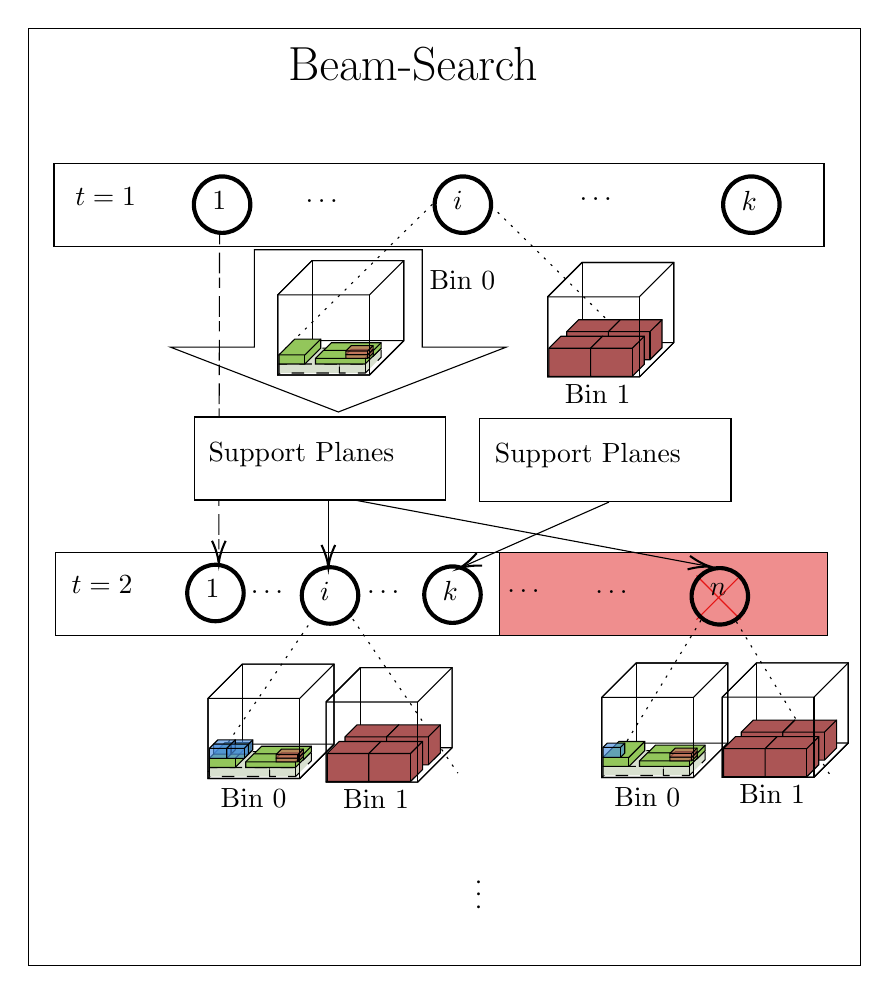
\begin{tikzpicture}[x=0.75pt,y=0.75pt,yscale=-1,xscale=1]
%uncomment if require: \path (0,540); %set diagram left start at 0, and has height of 540

%Right Arrow [id:dp8337745536636388] 
\draw   (281.86,136.75) -- (281.86,183.64) -- (322.31,183.64) -- (241.41,214.89) -- (160.5,183.64) -- (200.95,183.64) -- (200.95,136.75) -- cycle ;
%Straight Lines [id:da78157118634077] 
\draw  [dash pattern={on 3.75pt off 3pt on 7.5pt off 1.5pt}]  (184.2,129.1) -- (183.81,285.9) ;
\draw [shift={(183.8,287.9)}, rotate = 270.14] [color={rgb, 255:red, 0; green, 0; blue, 0 }  ][line width=0.75]    (10.93,-3.29) .. controls (6.95,-1.4) and (3.31,-0.3) .. (0,0) .. controls (3.31,0.3) and (6.95,1.4) .. (10.93,3.29)   ;
%Shape: Cube [id:dp22610144404804344] 
\draw   (272.94,180.54) -- (256.4,197.09) -- (212.23,197.09) -- (212.23,158.49) -- (228.77,141.94) -- (272.94,141.94) -- cycle ; \draw   (212.23,197.09) -- (228.77,180.54) -- (272.94,180.54) ; \draw   (228.77,180.54) -- (228.77,141.94) ;
%Shape: Rectangle [id:dp3675398368494672] 
\draw   (92,30) -- (493,30) -- (493,481.75) -- (92,481.75) -- cycle ;
%Shape: Rectangle [id:dp3872816319657796] 
\draw   (104.4,95) -- (475.4,95) -- (475.4,135) -- (104.4,135) -- cycle ;
%Straight Lines [id:da16266893569729468] 
\draw  [dash pattern={on 0.84pt off 2.51pt}]  (286.71,114.86) -- (211,189.14) ;
%Straight Lines [id:da2739363742069437] 
\draw  [dash pattern={on 0.84pt off 2.51pt}]  (315,115.5) -- (390.43,189.71) ;

%Shape: Cube [id:dp06723731454771065] 
\draw   (403,181.46) -- (386.46,198) -- (342.29,198) -- (342.29,159.4) -- (358.83,142.86) -- (403,142.86) -- cycle ; \draw   (342.29,198) -- (358.83,181.46) -- (403,181.46) ; \draw   (358.83,181.46) -- (358.83,142.86) ;
%Shape: Cube [id:dp9540002545180426] 
\draw  [fill={rgb, 255:red, 171; green, 85; blue, 85 }  ,fill opacity=1 ] (351.43,176.21) -- (357.21,170.43) -- (377.29,170.43) -- (377.29,183.93) -- (371.5,189.71) -- (351.43,189.71) -- cycle ; \draw   (377.29,170.43) -- (371.5,176.21) -- (351.43,176.21) ; \draw   (371.5,176.21) -- (371.5,189.71) ;
%Shape: Cube [id:dp4858900723039008] 
\draw  [fill={rgb, 255:red, 171; green, 85; blue, 85 }  ,fill opacity=1 ] (371.5,176.21) -- (377.29,170.43) -- (397.36,170.43) -- (397.36,183.93) -- (391.57,189.71) -- (371.5,189.71) -- cycle ; \draw   (397.36,170.43) -- (391.57,176.21) -- (371.5,176.21) ; \draw   (391.57,176.21) -- (391.57,189.71) ;
%Shape: Cube [id:dp37688563395090247] 
\draw  [fill={rgb, 255:red, 171; green, 85; blue, 85 }  ,fill opacity=1 ] (342.86,184.21) -- (348.64,178.43) -- (368.71,178.43) -- (368.71,191.93) -- (362.93,197.71) -- (342.86,197.71) -- cycle ; \draw   (368.71,178.43) -- (362.93,184.21) -- (342.86,184.21) ; \draw   (362.93,184.21) -- (362.93,197.71) ;
%Shape: Cube [id:dp29304074255321133] 
\draw  [fill={rgb, 255:red, 171; green, 85; blue, 85 }  ,fill opacity=1 ] (362.93,184.21) -- (368.71,178.43) -- (388.79,178.43) -- (388.79,191.93) -- (383,197.71) -- (362.93,197.71) -- cycle ; \draw   (388.79,178.43) -- (383,184.21) -- (362.93,184.21) ; \draw   (383,184.21) -- (383,197.71) ;
%Shape: Cube [id:dp012588700852047996] 
\draw   (342.29,159.4) -- (358.83,142.86) -- (403,142.86) -- (403,181.46) -- (386.46,198) -- (342.29,198) -- cycle ; \draw   (403,142.86) -- (386.46,159.4) -- (342.29,159.4) ; \draw   (386.46,159.4) -- (386.46,198) ;
%Shape: Cube [id:dp23988070590283161] 
\draw  [fill={rgb, 255:red, 216; green, 224; blue, 207 }  ,fill opacity=1 ][dash pattern={on 4.5pt off 4.5pt}] (212.84,191.76) -- (220.46,184.14) -- (249.52,184.14) -- (249.52,188.52) -- (241.9,196.13) -- (212.84,196.13) -- cycle ; \draw  [dash pattern={on 4.5pt off 4.5pt}] (249.52,184.14) -- (241.9,191.76) -- (212.84,191.76) ; \draw  [dash pattern={on 4.5pt off 4.5pt}] (241.9,191.76) -- (241.9,196.13) ;
%Shape: Cube [id:dp09035733009605551] 
\draw  [fill={rgb, 255:red, 216; green, 224; blue, 207 }  ,fill opacity=1 ][dash pattern={on 4.5pt off 4.5pt}] (241.9,191.76) -- (249.52,184.14) -- (262.04,184.14) -- (262.04,188.52) -- (254.42,196.13) -- (241.9,196.13) -- cycle ; \draw  [dash pattern={on 4.5pt off 4.5pt}] (262.04,184.14) -- (254.42,191.76) -- (241.9,191.76) ; \draw  [dash pattern={on 4.5pt off 4.5pt}] (254.42,191.76) -- (254.42,196.13) ;
%Shape: Cube [id:dp21044320148528428] 
\draw  [fill={rgb, 255:red, 147; green, 198; blue, 91 }  ,fill opacity=1 ] (212.84,187.39) -- (220.46,179.77) -- (232.93,179.77) -- (232.93,184.14) -- (225.31,191.76) -- (212.84,191.76) -- cycle ; \draw   (232.93,179.77) -- (225.31,187.39) -- (212.84,187.39) ; \draw   (225.31,187.39) -- (225.31,191.76) ;
%Shape: Cube [id:dp2634805119323166] 
\draw  [fill={rgb, 255:red, 147; green, 198; blue, 91 }  ,fill opacity=1 ] (234.29,185.34) -- (238.1,181.53) -- (262.04,181.53) -- (262.04,184.17) -- (258.22,187.99) -- (234.29,187.99) -- cycle ; \draw   (262.04,181.53) -- (258.22,185.34) -- (234.29,185.34) ; \draw   (258.22,185.34) -- (258.22,187.99) ;
%Shape: Cube [id:dp5335177162875748] 
\draw  [fill={rgb, 255:red, 147; green, 198; blue, 91 }  ,fill opacity=1 ] (230.41,189.08) -- (234.29,185.21) -- (258.16,185.21) -- (258.16,187.89) -- (254.29,191.76) -- (230.41,191.76) -- cycle ; \draw   (258.16,185.21) -- (254.29,189.08) -- (230.41,189.08) ; \draw   (254.29,189.08) -- (254.29,191.76) ;
%Shape: Cube [id:dp6236494259647203] 
\draw  [fill={rgb, 255:red, 198; green, 110; blue, 91 }  ,fill opacity=0.69 ] (245.05,187.29) -- (247.63,184.71) -- (258.16,184.71) -- (258.16,186.5) -- (255.58,189.08) -- (245.05,189.08) -- cycle ; \draw   (258.16,184.71) -- (255.58,187.29) -- (245.05,187.29) ; \draw   (255.58,187.29) -- (255.58,189.08) ;
%Shape: Cube [id:dp9516088630040508] 
\draw  [fill={rgb, 255:red, 198; green, 110; blue, 91 }  ,fill opacity=0.69 ] (245.05,185.5) -- (247.63,182.92) -- (258.16,182.92) -- (258.16,184.71) -- (255.58,187.29) -- (245.05,187.29) -- cycle ; \draw   (258.16,182.92) -- (255.58,185.5) -- (245.05,185.5) ; \draw   (255.58,185.5) -- (255.58,187.29) ;
%Shape: Cube [id:dp022246373009996434] 
\draw   (212.23,158.49) -- (228.77,141.94) -- (272.94,141.94) -- (272.94,180.54) -- (256.4,197.09) -- (212.23,197.09) -- cycle ; \draw   (272.94,141.94) -- (256.4,158.49) -- (212.23,158.49) ; \draw   (256.4,158.49) -- (256.4,197.09) ;
%Shape: Rectangle [id:dp6604290999676096] 
\draw  [fill={rgb, 255:red, 255; green, 255; blue, 255 }  ,fill opacity=1 ] (172,217.3) -- (293,217.3) -- (293,257.3) -- (172,257.3) -- cycle ;
%Shape: Rectangle [id:dp10394734829371921] 
\draw   (309.6,218.1) -- (430.6,218.1) -- (430.6,258.1) -- (309.6,258.1) -- cycle ;
%Shape: Rectangle [id:dp3884482964100383] 
\draw   (105.2,282.6) -- (476.2,282.6) -- (476.2,322.6) -- (105.2,322.6) -- cycle ;
%Shape: Rectangle [id:dp4662670618125976] 
\draw  [fill={rgb, 255:red, 239; green, 142; blue, 142 }  ,fill opacity=1 ] (319.2,282.5) -- (477,282.5) -- (477,322.5) -- (319.2,322.5) -- cycle ;
\draw  [color={rgb, 255:red, 229; green, 21; blue, 21 }  ,draw opacity=1 ] (413.99,293.69) -- (435.21,314.91)(435.21,293.69) -- (413.99,314.91) ;
%Straight Lines [id:da9423844633177114] 
\draw    (236.6,257.9) -- (236.6,287.9) ;
\draw [shift={(236.6,289.9)}, rotate = 270] [color={rgb, 255:red, 0; green, 0; blue, 0 }  ][line width=0.75]    (10.93,-3.29) .. controls (6.95,-1.4) and (3.31,-0.3) .. (0,0) .. controls (3.31,0.3) and (6.95,1.4) .. (10.93,3.29)   ;
%Straight Lines [id:da8187100513502555] 
\draw    (250.2,257.5) -- (419.03,289.13) ;
\draw [shift={(421,289.5)}, rotate = 190.61] [color={rgb, 255:red, 0; green, 0; blue, 0 }  ][line width=0.75]    (10.93,-3.29) .. controls (6.95,-1.4) and (3.31,-0.3) .. (0,0) .. controls (3.31,0.3) and (6.95,1.4) .. (10.93,3.29)   ;
%Straight Lines [id:da5112317799583161] 
\draw    (371.8,258.3) -- (301.23,289.49) ;
\draw [shift={(299.4,290.3)}, rotate = 336.16] [color={rgb, 255:red, 0; green, 0; blue, 0 }  ][line width=0.75]    (10.93,-3.29) .. controls (6.95,-1.4) and (3.31,-0.3) .. (0,0) .. controls (3.31,0.3) and (6.95,1.4) .. (10.93,3.29)   ;
%Shape: Cube [id:dp3098593802776677] 
\draw   (239.34,374.94) -- (222.8,391.49) -- (178.63,391.49) -- (178.63,352.89) -- (195.17,336.34) -- (239.34,336.34) -- cycle ; \draw   (178.63,391.49) -- (195.17,374.94) -- (239.34,374.94) ; \draw   (195.17,374.94) -- (195.17,336.34) ;
%Straight Lines [id:da052289940556063064] 
\draw  [dash pattern={on 0.84pt off 2.51pt}]  (229.41,314.06) -- (178.6,388.34) ;
%Straight Lines [id:da7979737763702788] 
\draw  [dash pattern={on 0.84pt off 2.51pt}]  (248.39,314.7) -- (299,388.91) ;

%Shape: Cube [id:dp563730868795463] 
\draw   (296.2,376.66) -- (279.66,393.2) -- (235.49,393.2) -- (235.49,354.6) -- (252.03,338.06) -- (296.2,338.06) -- cycle ; \draw   (235.49,393.2) -- (252.03,376.66) -- (296.2,376.66) ; \draw   (252.03,376.66) -- (252.03,338.06) ;
%Shape: Cube [id:dp6842297170502628] 
\draw  [fill={rgb, 255:red, 171; green, 85; blue, 85 }  ,fill opacity=1 ] (244.63,371.41) -- (250.41,365.63) -- (270.49,365.63) -- (270.49,379.13) -- (264.7,384.91) -- (244.63,384.91) -- cycle ; \draw   (270.49,365.63) -- (264.7,371.41) -- (244.63,371.41) ; \draw   (264.7,371.41) -- (264.7,384.91) ;
%Shape: Cube [id:dp36117121382423767] 
\draw  [fill={rgb, 255:red, 171; green, 85; blue, 85 }  ,fill opacity=1 ] (264.7,371.41) -- (270.49,365.63) -- (290.56,365.63) -- (290.56,379.13) -- (284.77,384.91) -- (264.7,384.91) -- cycle ; \draw   (290.56,365.63) -- (284.77,371.41) -- (264.7,371.41) ; \draw   (284.77,371.41) -- (284.77,384.91) ;
%Shape: Cube [id:dp5567622602150145] 
\draw  [fill={rgb, 255:red, 171; green, 85; blue, 85 }  ,fill opacity=1 ] (236.06,379.41) -- (241.84,373.63) -- (261.91,373.63) -- (261.91,387.13) -- (256.13,392.91) -- (236.06,392.91) -- cycle ; \draw   (261.91,373.63) -- (256.13,379.41) -- (236.06,379.41) ; \draw   (256.13,379.41) -- (256.13,392.91) ;
%Shape: Cube [id:dp9251910046018463] 
\draw  [fill={rgb, 255:red, 171; green, 85; blue, 85 }  ,fill opacity=1 ] (256.13,379.41) -- (261.91,373.63) -- (281.99,373.63) -- (281.99,387.13) -- (276.2,392.91) -- (256.13,392.91) -- cycle ; \draw   (281.99,373.63) -- (276.2,379.41) -- (256.13,379.41) ; \draw   (276.2,379.41) -- (276.2,392.91) ;
%Shape: Cube [id:dp97100963444055] 
\draw   (235.49,354.6) -- (252.03,338.06) -- (296.2,338.06) -- (296.2,376.66) -- (279.66,393.2) -- (235.49,393.2) -- cycle ; \draw   (296.2,338.06) -- (279.66,354.6) -- (235.49,354.6) ; \draw   (279.66,354.6) -- (279.66,393.2) ;
%Shape: Cube [id:dp3314229379764526] 
\draw  [fill={rgb, 255:red, 216; green, 224; blue, 207 }  ,fill opacity=1 ][dash pattern={on 4.5pt off 4.5pt}] (179.24,386.16) -- (186.86,378.54) -- (215.92,378.54) -- (215.92,382.92) -- (208.3,390.53) -- (179.24,390.53) -- cycle ; \draw  [dash pattern={on 4.5pt off 4.5pt}] (215.92,378.54) -- (208.3,386.16) -- (179.24,386.16) ; \draw  [dash pattern={on 4.5pt off 4.5pt}] (208.3,386.16) -- (208.3,390.53) ;
%Shape: Cube [id:dp4227409563137523] 
\draw  [fill={rgb, 255:red, 216; green, 224; blue, 207 }  ,fill opacity=1 ][dash pattern={on 4.5pt off 4.5pt}] (208.3,386.16) -- (215.92,378.54) -- (228.44,378.54) -- (228.44,382.92) -- (220.82,390.53) -- (208.3,390.53) -- cycle ; \draw  [dash pattern={on 4.5pt off 4.5pt}] (228.44,378.54) -- (220.82,386.16) -- (208.3,386.16) ; \draw  [dash pattern={on 4.5pt off 4.5pt}] (220.82,386.16) -- (220.82,390.53) ;
%Shape: Cube [id:dp9493780297339603] 
\draw  [fill={rgb, 255:red, 147; green, 198; blue, 91 }  ,fill opacity=1 ] (179.24,381.79) -- (186.86,374.17) -- (199.33,374.17) -- (199.33,378.54) -- (191.71,386.16) -- (179.24,386.16) -- cycle ; \draw   (199.33,374.17) -- (191.71,381.79) -- (179.24,381.79) ; \draw   (191.71,381.79) -- (191.71,386.16) ;
%Shape: Cube [id:dp20210982349003004] 
\draw  [fill={rgb, 255:red, 147; green, 198; blue, 91 }  ,fill opacity=1 ] (200.69,379.74) -- (204.5,375.93) -- (228.44,375.93) -- (228.44,378.57) -- (224.62,382.39) -- (200.69,382.39) -- cycle ; \draw   (228.44,375.93) -- (224.62,379.74) -- (200.69,379.74) ; \draw   (224.62,379.74) -- (224.62,382.39) ;
%Shape: Cube [id:dp6451220456842981] 
\draw  [fill={rgb, 255:red, 147; green, 198; blue, 91 }  ,fill opacity=1 ] (196.81,383.48) -- (200.69,379.61) -- (224.56,379.61) -- (224.56,382.29) -- (220.69,386.16) -- (196.81,386.16) -- cycle ; \draw   (224.56,379.61) -- (220.69,383.48) -- (196.81,383.48) ; \draw   (220.69,383.48) -- (220.69,386.16) ;
%Shape: Cube [id:dp3910721600427305] 
\draw  [fill={rgb, 255:red, 198; green, 110; blue, 91 }  ,fill opacity=0.69 ] (211.45,381.69) -- (214.03,379.11) -- (224.56,379.11) -- (224.56,380.9) -- (221.98,383.48) -- (211.45,383.48) -- cycle ; \draw   (224.56,379.11) -- (221.98,381.69) -- (211.45,381.69) ; \draw   (221.98,381.69) -- (221.98,383.48) ;
%Shape: Cube [id:dp23309754303051422] 
\draw  [fill={rgb, 255:red, 198; green, 110; blue, 91 }  ,fill opacity=0.69 ] (211.45,379.9) -- (214.03,377.32) -- (224.56,377.32) -- (224.56,379.11) -- (221.98,381.69) -- (211.45,381.69) -- cycle ; \draw   (224.56,377.32) -- (221.98,379.9) -- (211.45,379.9) ; \draw   (221.98,379.9) -- (221.98,381.69) ;
%Shape: Cube [id:dp4655482842473665] 
\draw   (178.63,352.89) -- (195.17,336.34) -- (239.34,336.34) -- (239.34,374.94) -- (222.8,391.49) -- (178.63,391.49) -- cycle ; \draw   (239.34,336.34) -- (222.8,352.89) -- (178.63,352.89) ; \draw   (222.8,352.89) -- (222.8,391.49) ;
%Shape: Cube [id:dp4152358812705026] 
\draw   (429.04,374.44) -- (412.5,390.99) -- (368.33,390.99) -- (368.33,352.39) -- (384.87,335.84) -- (429.04,335.84) -- cycle ; \draw   (368.33,390.99) -- (384.87,374.44) -- (429.04,374.44) ; \draw   (384.87,374.44) -- (384.87,335.84) ;
%Straight Lines [id:da6929539156017857] 
\draw  [dash pattern={on 0.84pt off 2.51pt}]  (416.13,315.26) -- (370.6,389.54) ;
%Straight Lines [id:da2520104054773419] 
\draw  [dash pattern={on 0.84pt off 2.51pt}]  (433.14,315.9) -- (478.5,390.11) ;

%Shape: Cube [id:dp30742448269234246] 
\draw   (487.1,374.36) -- (470.56,390.9) -- (426.39,390.9) -- (426.39,352.3) -- (442.93,335.76) -- (487.1,335.76) -- cycle ; \draw   (426.39,390.9) -- (442.93,374.36) -- (487.1,374.36) ; \draw   (442.93,374.36) -- (442.93,335.76) ;
%Shape: Cube [id:dp5547181392678717] 
\draw  [fill={rgb, 255:red, 171; green, 85; blue, 85 }  ,fill opacity=1 ] (435.53,369.11) -- (441.31,363.33) -- (461.39,363.33) -- (461.39,376.83) -- (455.6,382.61) -- (435.53,382.61) -- cycle ; \draw   (461.39,363.33) -- (455.6,369.11) -- (435.53,369.11) ; \draw   (455.6,369.11) -- (455.6,382.61) ;
%Shape: Cube [id:dp7714989563411607] 
\draw  [fill={rgb, 255:red, 171; green, 85; blue, 85 }  ,fill opacity=1 ] (455.6,369.11) -- (461.39,363.33) -- (481.46,363.33) -- (481.46,376.83) -- (475.67,382.61) -- (455.6,382.61) -- cycle ; \draw   (481.46,363.33) -- (475.67,369.11) -- (455.6,369.11) ; \draw   (475.67,369.11) -- (475.67,382.61) ;
%Shape: Cube [id:dp6802562603958051] 
\draw  [fill={rgb, 255:red, 171; green, 85; blue, 85 }  ,fill opacity=1 ] (426.96,377.11) -- (432.74,371.33) -- (452.81,371.33) -- (452.81,384.83) -- (447.03,390.61) -- (426.96,390.61) -- cycle ; \draw   (452.81,371.33) -- (447.03,377.11) -- (426.96,377.11) ; \draw   (447.03,377.11) -- (447.03,390.61) ;
%Shape: Cube [id:dp3575223135416413] 
\draw  [fill={rgb, 255:red, 171; green, 85; blue, 85 }  ,fill opacity=1 ] (447.03,377.11) -- (452.81,371.33) -- (472.89,371.33) -- (472.89,384.83) -- (467.1,390.61) -- (447.03,390.61) -- cycle ; \draw   (472.89,371.33) -- (467.1,377.11) -- (447.03,377.11) ; \draw   (467.1,377.11) -- (467.1,390.61) ;
%Shape: Cube [id:dp04583492087348129] 
\draw   (426.39,352.3) -- (442.93,335.76) -- (487.1,335.76) -- (487.1,374.36) -- (470.56,390.9) -- (426.39,390.9) -- cycle ; \draw   (487.1,335.76) -- (470.56,352.3) -- (426.39,352.3) ; \draw   (470.56,352.3) -- (470.56,390.9) ;
%Shape: Cube [id:dp22648598314600765] 
\draw  [fill={rgb, 255:red, 216; green, 224; blue, 207 }  ,fill opacity=1 ][dash pattern={on 4.5pt off 4.5pt}] (368.94,385.66) -- (376.56,378.04) -- (405.62,378.04) -- (405.62,382.42) -- (398,390.03) -- (368.94,390.03) -- cycle ; \draw  [dash pattern={on 4.5pt off 4.5pt}] (405.62,378.04) -- (398,385.66) -- (368.94,385.66) ; \draw  [dash pattern={on 4.5pt off 4.5pt}] (398,385.66) -- (398,390.03) ;
%Shape: Cube [id:dp11910803660750402] 
\draw  [fill={rgb, 255:red, 216; green, 224; blue, 207 }  ,fill opacity=1 ][dash pattern={on 4.5pt off 4.5pt}] (398,385.66) -- (405.62,378.04) -- (418.14,378.04) -- (418.14,382.42) -- (410.52,390.03) -- (398,390.03) -- cycle ; \draw  [dash pattern={on 4.5pt off 4.5pt}] (418.14,378.04) -- (410.52,385.66) -- (398,385.66) ; \draw  [dash pattern={on 4.5pt off 4.5pt}] (410.52,385.66) -- (410.52,390.03) ;
%Shape: Cube [id:dp03436669328315789] 
\draw  [fill={rgb, 255:red, 147; green, 198; blue, 91 }  ,fill opacity=1 ] (368.94,381.29) -- (376.56,373.67) -- (389.03,373.67) -- (389.03,378.04) -- (381.41,385.66) -- (368.94,385.66) -- cycle ; \draw   (389.03,373.67) -- (381.41,381.29) -- (368.94,381.29) ; \draw   (381.41,381.29) -- (381.41,385.66) ;
%Shape: Cube [id:dp3001366964737242] 
\draw  [fill={rgb, 255:red, 147; green, 198; blue, 91 }  ,fill opacity=1 ] (390.39,379.24) -- (394.2,375.43) -- (418.14,375.43) -- (418.14,378.07) -- (414.32,381.89) -- (390.39,381.89) -- cycle ; \draw   (418.14,375.43) -- (414.32,379.24) -- (390.39,379.24) ; \draw   (414.32,379.24) -- (414.32,381.89) ;
%Shape: Cube [id:dp9791091368910745] 
\draw  [fill={rgb, 255:red, 147; green, 198; blue, 91 }  ,fill opacity=1 ] (386.51,382.98) -- (390.39,379.11) -- (414.26,379.11) -- (414.26,381.79) -- (410.39,385.66) -- (386.51,385.66) -- cycle ; \draw   (414.26,379.11) -- (410.39,382.98) -- (386.51,382.98) ; \draw   (410.39,382.98) -- (410.39,385.66) ;
%Shape: Cube [id:dp5345838256134253] 
\draw  [fill={rgb, 255:red, 198; green, 110; blue, 91 }  ,fill opacity=0.69 ] (401.15,381.19) -- (403.73,378.61) -- (414.26,378.61) -- (414.26,380.4) -- (411.68,382.98) -- (401.15,382.98) -- cycle ; \draw   (414.26,378.61) -- (411.68,381.19) -- (401.15,381.19) ; \draw   (411.68,381.19) -- (411.68,382.98) ;
%Shape: Cube [id:dp8233627388074675] 
\draw  [fill={rgb, 255:red, 74; green, 144; blue, 226 }  ,fill opacity=0.66 ] (368.94,376.49) -- (370.99,374.44) -- (379.4,374.44) -- (379.4,379.24) -- (377.34,381.29) -- (368.94,381.29) -- cycle ; \draw   (379.4,374.44) -- (377.34,376.49) -- (368.94,376.49) ; \draw   (377.34,376.49) -- (377.34,381.29) ;
%Shape: Cube [id:dp3945702568476691] 
\draw  [fill={rgb, 255:red, 198; green, 110; blue, 91 }  ,fill opacity=0.69 ] (401.15,379.4) -- (403.73,376.82) -- (414.26,376.82) -- (414.26,378.61) -- (411.68,381.19) -- (401.15,381.19) -- cycle ; \draw   (414.26,376.82) -- (411.68,379.4) -- (401.15,379.4) ; \draw   (411.68,379.4) -- (411.68,381.19) ;
%Shape: Cube [id:dp8251331839204266] 
\draw   (368.33,352.39) -- (384.87,335.84) -- (429.04,335.84) -- (429.04,374.44) -- (412.5,390.99) -- (368.33,390.99) -- cycle ; \draw   (429.04,335.84) -- (412.5,352.39) -- (368.33,352.39) ; \draw   (412.5,352.39) -- (412.5,390.99) ;
%Shape: Cube [id:dp2708464120930435] 
\draw  [fill={rgb, 255:red, 74; green, 144; blue, 226 }  ,fill opacity=0.66 ] (189.7,374.94) -- (191.75,372.88) -- (200.16,372.88) -- (200.16,377.68) -- (198.1,379.74) -- (189.7,379.74) -- cycle ; \draw   (200.16,372.88) -- (198.1,374.94) -- (189.7,374.94) ; \draw   (198.1,374.94) -- (198.1,379.74) ;
%Shape: Cube [id:dp15483932168959624] 
\draw  [fill={rgb, 255:red, 74; green, 144; blue, 226 }  ,fill opacity=0.66 ] (181.29,374.94) -- (183.35,372.88) -- (191.75,372.88) -- (191.75,377.68) -- (189.7,379.74) -- (181.29,379.74) -- cycle ; \draw   (191.75,372.88) -- (189.7,374.94) -- (181.29,374.94) ; \draw   (189.7,374.94) -- (189.7,379.74) ;
%Shape: Cube [id:dp5792684196727304] 
\draw  [fill={rgb, 255:red, 74; green, 144; blue, 226 }  ,fill opacity=0.66 ] (179.24,376.99) -- (181.29,374.94) -- (189.7,374.94) -- (189.7,379.74) -- (187.64,381.79) -- (179.24,381.79) -- cycle ; \draw   (189.7,374.94) -- (187.64,376.99) -- (179.24,376.99) ; \draw   (187.64,376.99) -- (187.64,381.79) ;
%Shape: Cube [id:dp6982160774307449] 
\draw  [fill={rgb, 255:red, 74; green, 144; blue, 226 }  ,fill opacity=0.66 ] (187.64,376.99) -- (189.7,374.94) -- (198.1,374.94) -- (198.1,379.74) -- (196.04,381.79) -- (187.64,381.79) -- cycle ; \draw   (198.1,374.94) -- (196.04,376.99) -- (187.64,376.99) ; \draw   (196.04,376.99) -- (196.04,381.79) ;

% Text Node
\draw (216,38) node [anchor=north west][inner sep=0.75pt]   [align=left] {{\LARGE Beam-Search}};
% Text Node
\draw  [line width=1.5]   (185.4, 115) circle [x radius= 13.6, y radius= 13.6]   ;
\draw (179.4,107.4) node [anchor=north west][inner sep=0.75pt]    {$1$};
% Text Node
\draw (113.4,105.4) node [anchor=north west][inner sep=0.75pt]    {$t=1$};
% Text Node
\draw  [line width=1.5]   (301.4, 115) circle [x radius= 13.6, y radius= 13.6]   ;
\draw (295.4,107.4) node [anchor=north west][inner sep=0.75pt]    {$i$};
% Text Node
\draw  [line width=1.5]   (440.4, 115) circle [x radius= 13.6, y radius= 13.6]   ;
\draw (434.4,107.4) node [anchor=north west][inner sep=0.75pt]    {$k$};
% Text Node
\draw (224.4,111.4) node [anchor=north west][inner sep=0.75pt]    {$\dotsc $};
% Text Node
\draw (356.4,110.4) node [anchor=north west][inner sep=0.75pt]    {$\dotsc $};
% Text Node
\draw (284.09,145.3) node [anchor=north west][inner sep=0.75pt]   [align=left] {Bin 0};
% Text Node
\draw (349.26,200.23) node [anchor=north west][inner sep=0.75pt]   [align=left] {Bin 1};
% Text Node
\draw (177.6,228.1) node [anchor=north west][inner sep=0.75pt]   [align=left] {Support Planes};
% Text Node
\draw (315.6,228.5) node [anchor=north west][inner sep=0.75pt]   [align=left] {Support Planes};
% Text Node
\draw  [line width=1.5]   (182.2, 302.1) circle [x radius= 13.6, y radius= 13.6]   ;
\draw (176.2,294.5) node [anchor=north west][inner sep=0.75pt]    {$1$};
% Text Node
\draw (111.7,292.5) node [anchor=north west][inner sep=0.75pt]    {$t=2$};
% Text Node
\draw  [line width=1.5]   (237.4, 303.3) circle [x radius= 13.6, y radius= 13.6]   ;
\draw (231.4,295.7) node [anchor=north west][inner sep=0.75pt]    {$i$};
% Text Node
\draw  [line width=1.5]   (296.4, 302.9) circle [x radius= 13.6, y radius= 13.6]   ;
\draw (290.4,295.3) node [anchor=north west][inner sep=0.75pt]    {$k$};
% Text Node
\draw (198,299.7) node [anchor=north west][inner sep=0.75pt]    {$\dotsc $};
% Text Node
\draw (254,299.5) node [anchor=north west][inner sep=0.75pt]    {$\dotsc $};
% Text Node
\draw (321.6,299.1) node [anchor=north west][inner sep=0.75pt]    {$\dotsc $};
% Text Node
\draw  [line width=1.5]   (425.2, 303.7) circle [x radius= 13.6, y radius= 13.6]   ;
\draw (419.2,296.1) node [anchor=north west][inner sep=0.75pt]    {$n$};
% Text Node
\draw (364,299.5) node [anchor=north west][inner sep=0.75pt]    {$\dotsc $};
% Text Node
\draw (310.95,438.37) node [anchor=north west][inner sep=0.75pt]  [rotate=-89.78]  {$\dotsc $};
% Text Node
\draw (183.49,395.2) node [anchor=north west][inner sep=0.75pt]   [align=left] {Bin 0};
% Text Node
\draw (242.46,395.43) node [anchor=north west][inner sep=0.75pt]   [align=left] {Bin 1};
% Text Node
\draw (373.19,394.7) node [anchor=north west][inner sep=0.75pt]   [align=left] {Bin 0};
% Text Node
\draw (433.36,393.13) node [anchor=north west][inner sep=0.75pt]   [align=left] {Bin 1};


\end{tikzpicture}

    }
    \caption{Conceptual representation of the proposed heuristic}
    \label{fig:heur_scheme}
\end{figure}


We developed a new constructive heuristic for the single-bin 3D-BPP called Support Planes (SP).
This heuristic sequentially inserts items within the bin, placing them on top of other items already placed.
In this way, it is always possible to guarantee vertical support for the inserted items.
Given a set of already positioned items, we define the two-dimensional plane that rests on the top face of those items as a support plane. Each bin will have multiple support planes since each item is placed at different elevations and has different heights. Each support plane is identified by its coordinate on the vertical axis ($z$), has regions where there is no support from items below, and regions where it is not possible to place items without overlapping with other placed items.

The insertion of items into a bin is performed by solving a two-dimensional bin packing problem (2D-BPP) for each support plane. 
Such 2D-BPP takes into account regions without vertical support and regions with obstacles.
For each support plane, we test the insertion of each item. The plane is selected with a first-fit strategy starting from the lowest $z$, while the items to be inserted are selected with a best-fit strategy until the selected plane is filled.
The best-fit strategy is based on selecting items that can generate well-supported planes along with the already placed items. In addition, placements are also intended to avoid over-satisfying the support constraint, which could lead to unbalanced bins as reported in \cite{elhedhli2019three}.

To reduce the number of placements to consider, we propose two SP configurations: in the first, 2D-BPP is solved for single item placement (PS), while in the second, 2D-BPP is solved for placement of groups of items with the same dimensions (PM).
We solve the aforementioned 2D-BPP with a new modified version of the Extreme Points algorithm proposed in \cite{crainic2008extreme}.
In our implementation, we use several tricks to improve performance, such as the use of axis-align bounding box trees for fast collision checks (\cite{bergen1997efficient}).

Our studies have shown that choosing placements with a best-fit strategy does not achieve satisfactory solutions. For this reason, we extend our constructive heuristics with a beam-search algorithm. 
We define a solution as a set of open bins with their packed items. We say that a solution is partial if there are items that still need to be packed.
Our beam-search algorithm starts from the empty solution and iteratively explores $k$ new partial solutions.
These partial solutions are generated from the solutions of the previous iteration by applying SP. 
Whenever SP is not able to place items in the opened bins of a partial solution, a new bin is opened.
Since each new partial solution is obtained by inserting a positive amount of items in another partial solution, the algorithm will always converge to a set of solutions where no item is unpacked.
To limit the number of partial solutions considered at each iteration, we define a ranking between them, using metrics related to the objective function of our MILP model.
We rank these solutions considering the number of opened bins, the amount of packed volume, and the average cage ratio among opened bins.
Since different sequences of placements can lead to the same partial solution, we also developed a removal procedure that filters duplicate solutions based on a hashing function.


%-----------------------------------------------------------------------------
% CONCLUSION
%-----------------------------------------------------------------------------
\section{Conclusions}
In this thesis, we presented a heuristic for the Three-Dimensional Bin Packing Problem with Vertical Support.
We modified the two-dimensional Extreme Points algorithm of \citet{crainic2008extreme} to consider vertical support.
We then used this modified algorithm in a constructive heuristic which builds solutions to the single bin three-dimensional bin packing problem by filling planes generated based on the previously inserted items.
Finally, we introduced a beam-search algorithm that evaluates different sequences of item placements by using our proposed constructive heuristic and removes duplicate solutions at each iteration.

We tested a relaxed version of our heuristic without the support constraint and the rotation of items on the benchmark instances for the 3D-BPP proposed by \cite{martello2000three}.
Our heuristic achieved an average gap of $5.37\%$ against the best solutions in the literature; however, we were able to solve the same instances in a fraction of their computational time.
We consider this a great result since it states that our algorithm is also competitive in the realm of 3D-BPP without support.
We generated a data set of problem instances based on real-world products from our case study, and we used them to evaluate our heuristic.
Our solutions exceeded the target metric of $70\%$ cage ratio in most configurations, with some of them having a negligible execution time.
In \cref{results:usecase_summary} we report the average execution time (\textit{TT}) in milliseconds, number of opened bins (B), and cage ratio (\textit{CR}) across all our case study instances. Each row of the table reports the aggregated results on all instances with different value of $k$.
Different placement modes are marked as PS (single placement) and PM (multiple items per placement).
In \cref{exp:usecase_tradeoff} we analyze the trade-off between running times and cage ratio obtained by each configuration of the heuristic.
We list the difference between the average running time of each configuration (\textit{TT}) and the best average running time (\textit{TT*}), together with the difference between the best average cage ratio (\textit{CR*}) and the average cage ratio obtained by each configuration (\textit{CR}).
We discover that the most promising configuration for our industrial partner consists in using the PM placement mode with $k \in {20, 50}$.

Further research could introduce new practical constraints such as family groupings, load-bearing, and compatibility between items.
Improvement heuristics could also be adapted to account for vertical support, such as the space defragmentation techniques introduced by \cite{ZHU2012452}.

\begin{table}[htbp]
    \centering
    \caption{Summary of case study tests}
    \resizebox{\columnwidth}{!}{\begin{tabular}{|c|c|c|c|c|c|c|}
    \hline
    & \multicolumn{ 3}{c|}{\textbf{PS}} & \multicolumn{ 3}{c|}{\textbf{PM}} \\ \hline
    \textbf{$k$} & \textbf{\textit{TT (ms)}} & \textbf{\textit{B}} & \textbf{\textit{CR (\%)}} & \textbf{\textit{TT (ms)}} & \textbf{\textit{B}} & \textbf{\textit{CR (\%)}} \\ \hline
    $1$ & 423.87 & 1.37 & 65.87 & 65.18 & 1.31 & \textbf{70.70} \\ 
    $5$ & 1,597.54 & 1.34 & 69.19 & 185.22 & 1.29 & \textbf{73.08} \\ 
    $10$ & 2,627.52 & 1.32 & 70.35 & 344.90 & 1.27 & \textbf{73.56} \\ 
    $20$ & 5,373.79 & 1.34 & 70.78 & 620.95 & 1.27 & \textbf{74.57} \\ 
    $50$ & 14,203.10 & 1.31 & 72.11 & 1,279.96 & 1.29 & \textbf{74.61} \\ 
    $100$ & 26,934.21 & 1.31 & 73.23 & 2,340.37 & 1.26 & \textbf{75.36} \\ 
    $200$ & 48,944.90 & 1.30 & 73.89 & 4,465.78 & 1.25 & \textbf{76.39} \\ \hline
    \end{tabular}}
    \label{results:usecase_summary}
    \end{table}
    
\begin{table}[htbp]
    \caption{Case study experiments trade off between average execution times and average cage ratio}
    \centering
    \resizebox{\columnwidth}{!}{\begin{tabular}{|c|c|c|c|c|}
    \hline
    \multicolumn{1}{|c|}{\textbf{$k$}} & \multicolumn{ 2}{c|}{\textbf{\textit{PS}}} & \multicolumn{ 2}{c|}{\textbf{\textit{PM}}} \\ \hline
    \multicolumn{1}{|c|}{} & $\textbf{\textit{CR}} - \textbf{\textit{CR*}}$ \textbf{\textit{(\%)}} & $\textbf{\textit{TT}} - \textbf{\textit{TT* (ms)}}$ & $\textbf{\textit{CR}} - \textbf{\textit{CR*}}$ \textbf{\textit{(\%)}} & $\textbf{\textit{TT}} - \textbf{\textit{TT* (ms)}}$ \\ \hline
    1 & 10.56 & 358.69 & 5.73 & 0.00 \\
    5 & 7.24 & 1,532.36 & 3.35 & 120.04 \\
    10 & 6.08 & 2,562.34 & 2.87 & 279.72 \\
    \textbf{20} & 5.65 & 5,308.61 & \textbf{1.85} & \textbf{555.77} \\
    \textbf{50} & 4.32 & 14,137.92 & \textbf{1.82} & \textbf{1,214.78} \\
    100 & 3.20 & 26,869.03 & 1.07 & 2,275.19 \\
    200 & 2.54 & 48,879.72 & 0.04 & 4,400.60 \\ \hline
    \end{tabular}~}
    \label{exp:usecase_tradeoff}
\end{table}
    

\begin{figure}
    \centering
    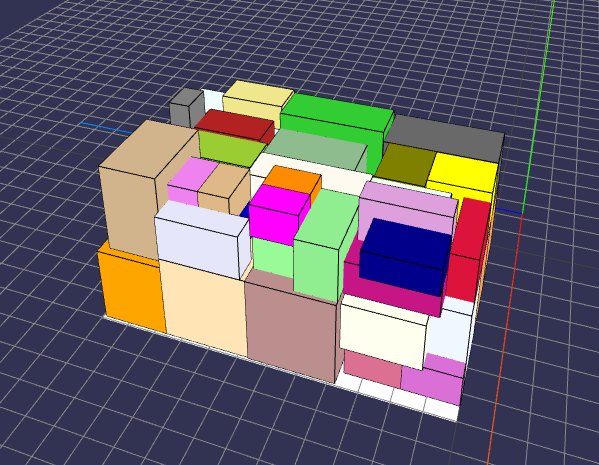
\includegraphics[width = \columnwidth]{tests/usecase/instance-82_k200.PNG}
    \caption{Solution to Instance 82 from case study tests}
\end{figure}

\begin{figure}
    \centering
    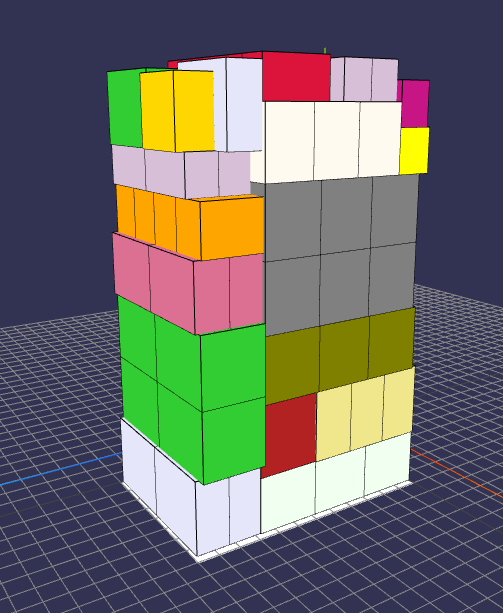
\includegraphics[width = \columnwidth]{tests/usecase/instance-66_bin1_k200.PNG}
    \caption{Solution to Instance 66, Bin 1 from case study tests}
\end{figure}

%---------------------------------------------------------------------------
%  ACKNOWLEDGEMENTS 
%---------------------------------------------------------------------------
\section{Acknowledgements}
My deepest gratitude goes to my supervisors, Prof. Ola Jabali and Dr. Davide Croci for their insights and support.
This work wouldn't have been possible without them.\\
\\
Thanks to the team at ERMES-X s.r.l who provided me with the case study and the data used for our experiments.\\
\\
Many thanks to my family, my mom Patrizia, my father Severino, and my sister Giulia for always supporting me during this journey.
Last but not least, thanks to my colleagues Alberto, Edoardo, Mirko, and Kevin, that brightened every day at the university.

%---------------------------------------------------------------------------
%  BIBLIOGRAPHY
%---------------------------------------------------------------------------
% Remember to insert here only the essential bibliography of your work
\setcitestyle{numbers} % set the citation style to ``numbers''.
\bibliography{literature.bib} % automatically inserted and ordered with this command 

\end{document}